\subsubsection{Adquirir los datos $M_{21}$}

En este módulo del sistema, se realiza la lectura de las sensores para las diferentes variables físicas que se van a observar durante el funcionamiento del sistema de compostaje. En esta parte se analiza y se selecciona el sensor que más se adapta a las necesidades. 

\textbf{Sensor de temperatura}

Para medir de temperatura se considero encontrar un dispositivo que funcione bajo ambientes corrosivos, que se pueda integrar a la tarjeta de desarrollo y que sea accesible. Con estos requisitos se optó por utilizar el sensor electrónico de semiconductor.

%Dentro de las desventajas, se encuentra que diversos sensores pueden sufrir perturbaciones en la composición de sus componentes conforme se exponen a temperaturas más altas, además de que muy poco empaquetados con capaces de resistir en ambientes tan corrosivos, como el que se plantea tener al interior del contenedor. 

Dentro de una lista de dispositivos comerciales,  se seleccionó el sensor DS18B20, este sensor está hecho a base de semiconductores. Este sensor esta integrado dentro del entorno de desarrollo de Arduino, por lo que su integración con la ESP 32 esta garantizada.

Otra ventaja, es que este sensor cuenta con una versión sumergible, que posee una cubierta  impermeable de acero inoxidable, de esta manera el sensor puede trabajar bajo condiciones de humedad que no afectan su funcionamiento, además de protegerlo de la corrosión.  Los detalles técnicos del sensor son los que describen en la tabla \ref{tab:Sensortem}

\begin{table}[h!]
    \centering
    \caption{Características del sensor DS18B20}
        \begin{tabular}{ |c|c|c|c| } 
            \hline
            \multirow{7}{8em}{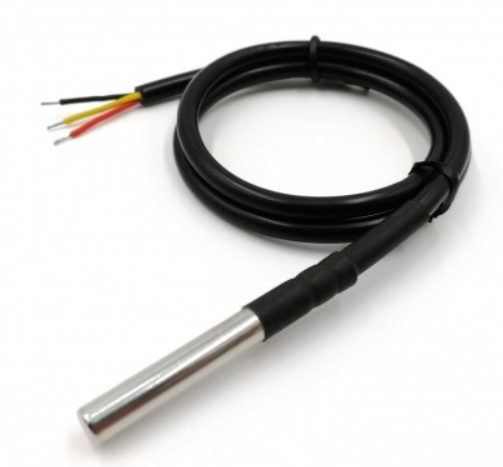
\includegraphics[scale=0.15]{images/Capitulo 4/S2/temperatura.png}} & \cellcolor[rgb]{ .851,  .851,  .851}Alimentación & \cellcolor[rgb]{ .851,  .851,  .851}3.0 a 5 V \\ 
            & Resolución & 9 a 12 bit \\ 
            & \cellcolor[rgb]{ .851,  .851,  .851}Rango de temperatura & \cellcolor[rgb]{ .851,  .851,  .851}50 a 125 C \\ 
            & Diámetro de la probeta & 6 a 9 mm \\
            & \cellcolor[rgb]{ .851,  .851,  .851}Largo de la probeta & \cellcolor[rgb]{ .851,  .851,  .851}10 a 1000 mm \\
            & Material de la probeta & Acero inoxidable \\
            & \cellcolor[rgb]{ .851,  .851,  .851}Conector & \cellcolor[rgb]{ .851,  .851,  .851}Molex, DuPont, CWB, CJT, U type\\
             \hline
        \end{tabular}
    \label{tab:Sensortem}%
\end{table}

\textbf{Sensor de humedad}

Para la medición de la humedad, se tomaron en cuenta dos tipos de sensores, los sensores que tienen contacto con la materia orgánica y los sensores que miden la humedad del ambiente. Para efectos de este trabajo, se ha seleccionado el sensor que mide la humedad del ambiente dentro del tanque del compostador.

Para esta parte se optó por utilizar el sensor de humedad y temperatura DHT11, este es un sensor electrónico que capta la humedad del ambiente y es capaz de mandar una señal digital con toda la información que ha captado. 

Este dispositivo también cuenta con una librería en el entorno de desarrollo de arduino, por lo que su integración con la tarjeta de desarrollo esta garantizada, además de que es un dispositivo económico, que según los antecedentes revisados en la tabla \ref{tab:Antecedentes}, tiene buen desempeño en este tipo de sistemas de compostajes. 

Las características del sensor, aparecen en la tabla \ref{tab:Sensorhum}

\begin{table}[h!]
    \centering
    \caption{Características del sensor DHT11}
        \begin{tabular}{ |c|c|c|c| } 
            \hline
            \multirow{6}{8em}{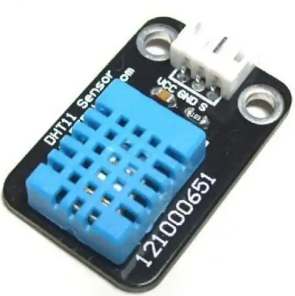
\includegraphics[scale=0.25]{images/Capitulo 4/S2/Humedad.png}} & \cellcolor[rgb]{ .851,  .851,  .851}Alimentación & \cellcolor[rgb]{ .851,  .851,  .851}3.0 a 5.5 V \\ 
            & Resolución & 1\% a 8 bit \\ 
            & \cellcolor[rgb]{ .851,  .851,  .851}Rango de humedad & \cellcolor[rgb]{ .851,  .851,  .851}20 a 80 \% \\ 
            & Tiempo de respuesta & 6 a 10 s \\
            & \cellcolor[rgb]{ .851,  .851,  .851}Señal de salida & \cellcolor[rgb]{ .851,  .851,  .851} Digital \\
            & \cellcolor[rgb]{ .851,  .851,  .851}Conector & \cellcolor[rgb]{ .851,  .851,  .851}DuPont\\
             \hline
        \end{tabular}
    \label{tab:Sensorhum}%
\end{table}
